\documentclass[12pt]{article}
\usepackage{sbc-template}
\usepackage{graphicx,url}
\usepackage[brazil]{babel}
\usepackage[utf8]{inputenc}
\usepackage{paralist}
\usepackage{graphicx}
\usepackage{subfig}
\usepackage{tabularx}
\usepackage{amsmath}
\usepackage{amssymb}
\usepackage{mathabx}

\sloppy

\title{Detecção de padrões de legendas em imagens de ritmo visual a partir
do detector de Harris}

\author{Guilherme Polo\inst{1}, Miguel Gaiowski\inst{1}}

\address{Instituto de Computação -- Universidade Estadual de Campinas
  (UNICAMP)\\
  Caixa Postal 6176 -- 13083-852 -- Campinas -- SP -- Brazil
  \email{\{ggpolo,miggaiowski\}@gmail.com}
}


\begin{document}
\maketitle

\begin{resumo}
  Este trabalho faz,  inicialmente, um resumo do detector  de cantos e
  bordas de  Harris.  Com  esse detector partimos  para a  extração de
  legendas  em  imagens  de  ritmo visual.   Descrevemos  sete  etapas
  complementares à Harris que  fornecem resultados razoáveis para esse
  tipo de imagem. Em especial,  aquelas onde o contraste entre regiões
  de legenda e demais partes  da imagem são mais perceptíveis foi onde
  nosso trabalho apresentou melhores resultados.
\end{resumo}


\section{Introdução}

A
\cite{harris}

B

C

D

E

F

G


\section{O detector de Harris}

A partir de  problemas existentes no detector de  Moravec, definido em
\cite{moravec},  surge o  detector  de Harris  \cite{harris}. A  ideia
básica desse detector  é conseguir indicar, ao mesmo  tempo, pontos de
canto e de  borda com o cálculo de uma  matriz que fornece informações
locais em cada pixel da imagem.

% XXX Pensando ...  O  detector de Harris \cite{harris} é classificado
% como um  método baseado  em intensidade \cite{detectors}.   capaz de
% indicar pontos de borda e canto em uma imagem. Ele parte do detector
% de Moravec \cite{moravec} e descreve diversas melhorias sobre aquele


Para definir essa matriz utilizada em Harris, primeiro consideramos uma
imagem $I$ e uma máscara $w$  como dadas. A máscara pode ser calculada
como   $w_{u,v}  =   \exp   -\frac{u^2  +   v^2}{2\sigma^2}$  --   uma
gaussiana. Com isso, essa matriz é inicialmente definida como:
\[
M = \begin{bmatrix}
  A & C \\
  C & B
\end{bmatrix}
\]
com
% Produto de Hadamard: \circ
\begin{align*}
  X & = I \convolution [-1, 0, 1] \\
  Y & = I \convolution [-1, 0, 1]^\intercal \\
  A & = (X \circ X) \convolution w \\
  B & = (Y \circ Y) \convolution w \\
  C & = (X \circ Y) \convolution w
\end{align*}
sendo $f \convolution h$ a  representação da convolução de $f$ com $h$
e  $M_1  \circ  M_2$  sendo  o  produto  de  Hadamard  que  realiza  a
multiplicação ponto a ponto entre as matrizes $M_1$ e $M_2$.

As matrizes $X$ e $Y$ descrevem, respectivamente, uma aproximação para
o  gradiente  em  $x$  e  em   $y$  da  imagem  $I$.   De  acordo  com
\cite{harris},  os autovalores  $\alpha$ e  $\beta$ da  matriz  $M$ --
considerando  um pixel  da imagem  -- capturam  a descrição  de cantos
($\alpha$ e $\beta$ são grandes),  bordas ($\alpha$ é grande e $\beta$
é pequeno,  ou vice-versa)  e regiões planas  ($\alpha$ e  $\beta$ são
pequenos).

Harris e  Stephens [1988],  então, procedem para  a construção  de uma
matriz $R$:  % XXX  Parece que  não da pra  fazer citeonline  com esse
% estilo.

\begin{align}
  Tr & = \alpha + \beta = A + B \nonumber \\
  Det & = \alpha \beta = A \circ B - C \circ C \nonumber \\
  R & = Det - k (Tr \circ Tr) \label{REq}
\end{align}

A  matriz formada  na  Equação  \ref{REq} define  todos  os pontos  de
interesse que esse detector consegue  capturar. O valor de $k$ não foi
estabelecido  no   trabalho  original  \cite{harris},   mas  trabalhos
variados \cite{detectors, statharris} mencionam valores entre $0,04$ e
$0,06$.   Neste trabalho fixamos  $k =  0,05$.  Nessa  matriz, valores
positivos são tomados como cantos, os negativos como bordas. Na figura
\ref{figR} há uma representação visual da matriz $R$.

\begin{figure}[h]
  \centering
  \subfloat{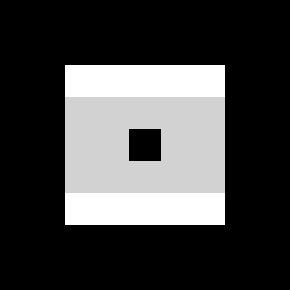
\includegraphics[height=4cm]{figs/sample_9_9.png}}\quad
  \subfloat{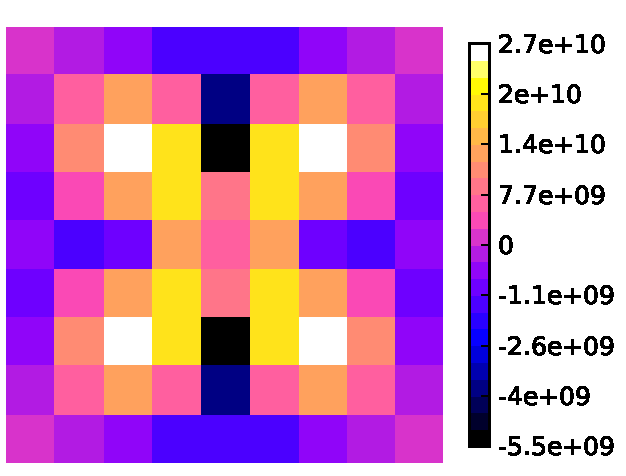
\includegraphics[height=4cm]{figs/sample_9_9_R}}
  \caption{Uma imagem 9x9 e sua respectiva matriz $R$ representada
    como um \textit{heatmap}\label{figR}}
\end{figure}

É possível distinguir facilmente os  pontos definidos como borda e como
cantos no \textit{heatmap} da Figura \ref{figR}. Os dois pontos pretos
são borda, enquanto que os  quatro brancos são cantos. Apesar de haver
diversos outros  pontos positivos  e negativos naquela  figura, Harris
ainda faz, conforme apresentado a seguir, duas considerações que levam
a esse conjunto de apenas seis pontos.

As Equações \ref{cornerEq} e \ref{edgeEq} definem, respectivamente, os
conjuntos de  pontos de canto  e de borda  com base na matriz  $R$. As
coordenadas $x$  e $y$ que  não pertencem a  $R$ são tomadas  como não
definidas.

\begin{align}
  &\{(x, y) \mid \forall R[x,y] > 0 \bullet R[x,y] = \max(R[x-1:x+1,y-1:y+1)\} \label{cornerEq} \\
  &\{
    (x, y) \mid \forall R[x,y] < 0 \bullet \mbox{} \nonumber \\
  & \quad\quad\quad R[x,y] < \left\{
      \begin{array}{l l}
        min(R[x-1,y], R[x+1,y]) & \mbox{se} \,\, A[x,y] > B[x,y]\\
        min(R[x,y-1], R[x,y+1]) & \mbox{c.c.}\\
      \end{array}
    \right. \label{edgeEq} \\
  &\} \nonumber
\end{align}

Na Equação \ref{cornerEq},  os pontos de canto que  não são máximos em
sua vizinhança direta são descartados.  No caso dos pontos de borda, a
Equação  \ref{edgeEq} indica que  só serão  bordas aqueles  pontos que
forem  mínimos onde  seu gradiente  é máximo  -- resultando  em bordas
finas.

\section{Implementação}

Com a matriz  $R$ (Equação \ref{REq}) construída e  os pontos de canto
(Equação  \ref{cornerEq}) e  borda  (Equação \ref{edgeEq})  definidos,
realizamos  mais sete  etapas  na expectativa  de  definir regiões  de
legenda  em imagens  de ritmo  visual. Na  primeira, a  partir  de uma
percentagem  do maior  valor em  $R$  descartamos os  pontos de  canto
inferiores a  este valor. Na  segunda, definimos um limiar  inferior e
outro  superior --  também com  base numa  percentagem do  maior valor
absoluto de ponto de borda --  para os pontos de borda e classificamos
cada  borda de  acordo  com  estes limiares  para,  então, realizar  a
histerese   \cite{snakebook}.   Estas   duas   primeiras  etapas   são
realizadas em cada banda da imagem e os resultados são combinados numa
única  imagem.  A  imagem resultante  até este  passo é  formada pelas
bordas  e cantos escolhidas,  com os  cantos sendo  representados como
quadrados 3x3 centrados no ponto de canto real.

A partir deste ponto,  são feitas tentativas para completar retângulos
quase fechados  que possivelmente  representam regiões de  legenda nas
imagens  de ritmo  visual. Para  cada  ponto ainda  não preenchido,  é
verificado  se  ambos seus  vizinhos  imediatos  na  horizontal ou  na
vertical foram preenchidos.  Caso ambos  em pelo menos uma das direções
tenham sido, este ponto não preenchido é marcado para preenchimento no
final deste processo.

Em  seguida,  o  algoritmo  \textit{flood  fill} é  aplicado  para  as
direções  horizontais e verticais  partindo do  ponto $(0,  0)$. Nesta
implementação, este ponto, garantidamente, é inicialmente preto devido
a não  consideração dos pontos em  $R$, para construir  as imagens até
este momento, onde a máscara gaussiana escolhida não esta inteiramente
contida na imagem (considerando a convolução no domínio espacial).

Na  quinta  etapa,  os  pontos  que permaneceram  pretos  são  aqueles
contidos dentro de formas fechadas. Com isso, uma nova imagem é criada
para apresentar  aqueles pontos pretos  agora como brancos.   Todos os
pontos brancos  nesta imagem formam  as possíveis regiões  de legenda.
Em seguida  é feita  uma filtragem da  mediana para  eliminar pequenas
regiões que  permaneceram devido a grande  heterogeneidade das imagens
de ritmo visual.

Finalmente,  na  sétima  etapa,   um  processamento  um  tanto  quanto
heurístico é  feito.  Cada região  branca da imagem é  considerada uma
componente conexa e  é feita, então, a contagem de  pixels em cada uma
dessas  componentes.  Aquelas  componentes  de tamanho  inferior a  um
valor estabelecido  são desconsideradas  na imagem final.   Isso acaba
limpando muitos fragmentos que sobreviveram até aqui.

\section{Avaliação}

Para realizar a  avaliação, os parâmetros foram fixados  para todos os
testes da  maneira seguinte: máscara  gaussiana 3x3 com $\sigma  = 2$,
limiar para pontos de  canto = $0.5 (\frac{max(R)}{100})$, limiares $H
= 2  (\frac{|min(R)|}{100})$ e $L =  0.01 (\frac{|min(R)|}{100})$ para
histerese,  máscara  5x5  para  filtragem  da mediana  e  descarte  de
componentes de tamanho inferior a 20 pixels.

De modo geral,  o detector de Harris, com  os demais passos aplicados,
foi capaz de encontrar regiões de legenda quando estas apresentavam um
contraste   adequado   na   imagem   como   um   todo.    As   Figuras
\ref{lowcontrast}   e  \ref{highcontrast}   apresentam   um  resultado
considerado, por nós, ruim e bom, respectivamente.

\begin{figure}[h!]
  \centering
  \subfloat{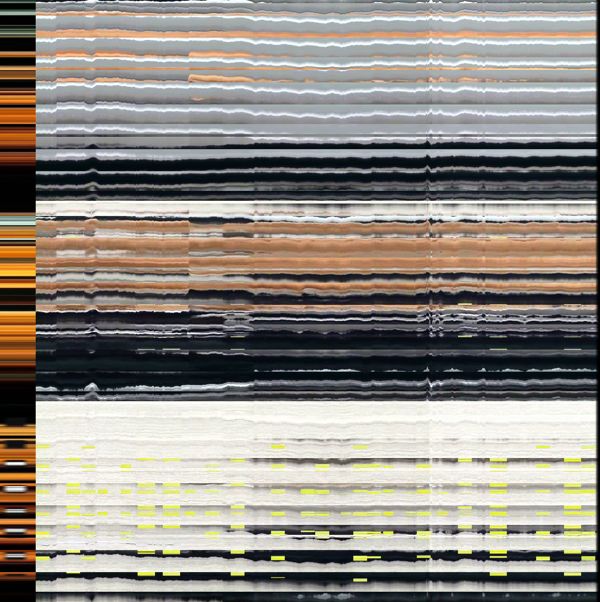
\includegraphics[width=0.45\linewidth]{figs/cats2.png}}\quad
  \subfloat{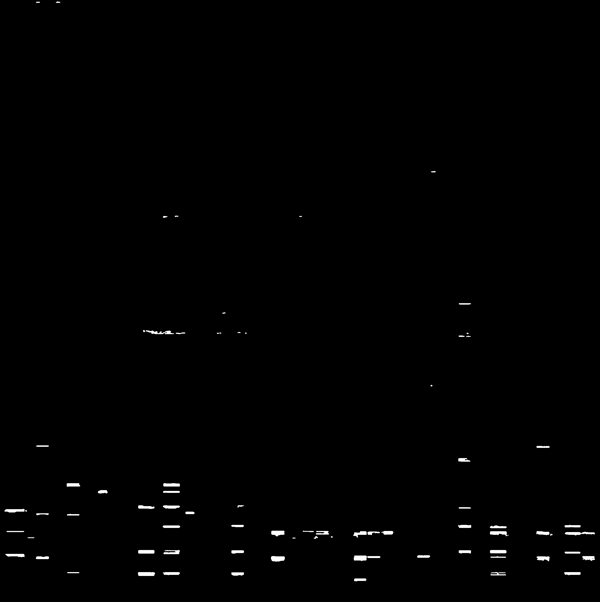
\includegraphics[width=0.45\linewidth]{figs/cats2_result.png}}
  \caption{Muitas regiões de legenda perdidas\label{lowcontrast}}
\end{figure}

\begin{figure}[h!]
  \centering
  \subfloat{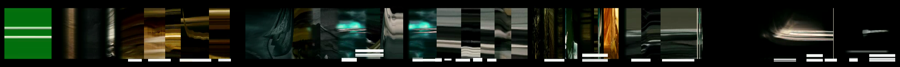
\includegraphics[width=\linewidth]{figs/harrypotter1.png}}\quad
  \subfloat{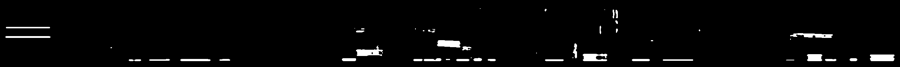
\includegraphics[width=\linewidth]{figs/harrypotter1_result.png}}
  \caption{Grande parte das regiões de legenda encontradas; alguns
    erros\label{highcontrast}}
\end{figure}

Na  Figura \ref{lowcontrast}, acreditamos  que cerca  de seu  um terço
superior não apresente legendas  e nosso método detecta poucas regiões
nessa  área.  % Entretanto,  no   segundo  terço  o   método  apresenta
% falso-positivos em excesso. %% Não é mais valido com a última etapa.
Na última parte  desta imagem é onde grande  parte das legendas estão,
mas  a  taxa   de  acerto  foi  baixa.   Por   outro  lado,  a  Figura
\ref{highcontrast}  apresenta o  caso  em que  nosso  método tem  bons
resultados.   Apesar de  reportar incorretamente  algumas  partes como
sendo  de legenda,  todas  as  reais regiões  de  legenda foram  quase
completamente indicadas.

\begin{figure}[h!]
  \centering
  \subfloat{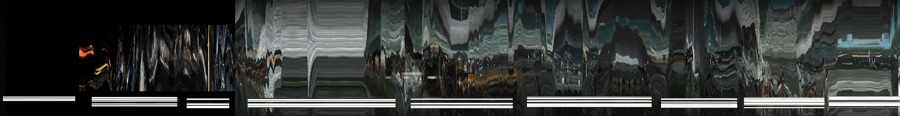
\includegraphics[width=\linewidth,height=1cm]{figs/t1_p1.png}}\quad
  \subfloat{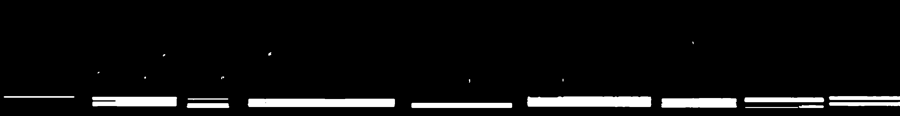
\includegraphics[width=\linewidth,height=1cm]{figs/t1r_p1.png}}\\
  \subfloat{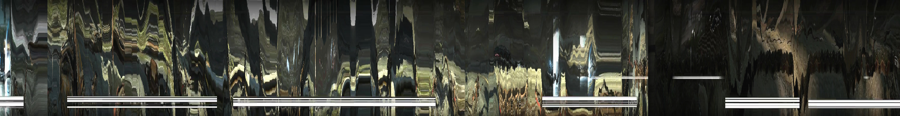
\includegraphics[width=\linewidth,height=1cm]{figs/t1_p2.png}}\quad
  \subfloat{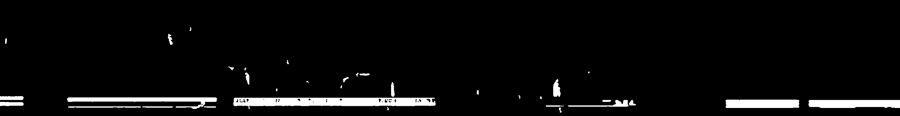
\includegraphics[width=\linewidth,height=1cm]{figs/t1r_p2.png}}\\
  \subfloat{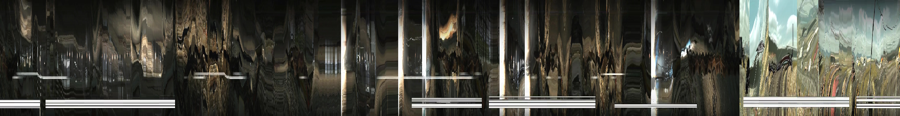
\includegraphics[width=\linewidth,height=1cm]{figs/t1_p3.png}}\quad
  \subfloat{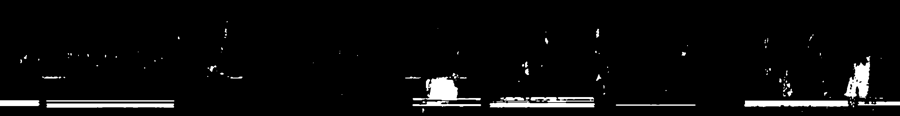
\includegraphics[width=\linewidth,height=1cm]{figs/t1r_p3.png}}\\
  \subfloat{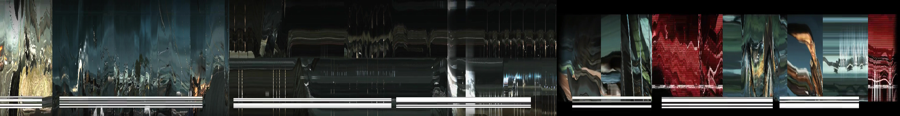
\includegraphics[width=\linewidth,height=1cm]{figs/t1_p4.png}}\quad
  \subfloat{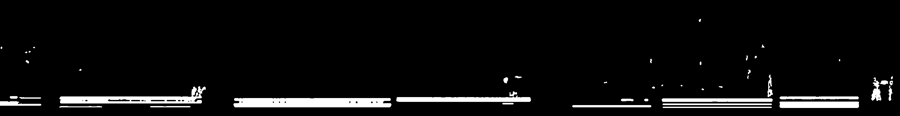
\includegraphics[width=\linewidth,height=1cm]{figs/t1r_p4.png}}\\
  \caption{Maioria das regiões de legendas foram reportadas\label{highcontrast2}}
\end{figure}

A  Figura \ref{highcontrast2}  apresenta  uma imagem  de ritmo  visual
significantemente maior  que aquela da  Figura \ref{highcontrast}. Ela
suporta  nossa suposição  em  relação ao  contraste  entre legendas  e
imagem como um todo.


\section{Conclusão}

Um  dos pontos a  ser discutido  é o  fato de  que, em  certas imagens
testadas, nem  mesmo humanos  (nós autores) conseguem  identificar com
absoluta  certeza a  posição das  legendas.  É difícil  esperar de  um
algoritmo  um  trabalho que  sequer  há  certeza  sobre os  resultados
esperados. Mesmo assim, em vários casos foi possível guiar o algoritmo
através  de ajustes  de parâmetros  e consertos  de detalhes  para que
chegasse em resultados aparentemente satisfatórios.

Como detector de bordas, Harris é um bom detector de cantos. % :)
Para a  tarefa de encontrar legendas  nas imagens de  ritmo visual ele
serviu  apenas como  um passo  0,  sendo discutível  se os  resultados
seguintes não  teriam sido  melhores com uso  de outro  detector.  Uma
quantidade razoável  de algoritmos heurísticos  foram implementados em
conjunto para produzir algum resultado parcialmente adequado.

O  número de  linhas de  código para  a implementação  do  detector de
Harris  é mínima quando  comparada ao  resto do  programa. De  fato, a
maior parte do trabalho foi feita por processos posteriores.
% Uma crítica é  que talvez fosse possível fazer a  mesma coisa, com a
% mesma quantidade de linhas de código, sem usar Harris.
Além  disso,  muitos  parâmetros   precisam  ser  definidos  de  forma
quase arbitrária.


\bibliographystyle{sbc}
\bibliography{biblio}

\end{document}
